% --- PREAMBULO (pdflatex) ---
\documentclass[11pt, a4paper]{article}
\usepackage[a4paper, top=2.5cm, bottom=2.5cm, left=2cm, right=2cm]{geometry}
\usepackage[T1]{fontenc}
\usepackage[utf8]{inputenc}
\usepackage{lmodern}
\usepackage{amsmath}
\usepackage{array}
\usepackage{booktabs}
\usepackage{xcolor}
\usepackage{graphicx}
\graphicspath{{./}}
\usepackage{fancyhdr}
\usepackage{titlesec}
\usepackage{lastpage}
\usepackage[section]{placeins}
\usepackage[hidelinks]{hyperref}
\usepackage[spanish, es-tabla]{babel}

\usepackage{enumitem}
\setlist[itemize]{label=-}

% Paleta
\definecolor{primary}{HTML}{0F172A}
\definecolor{alertred}{HTML}{DC2626}
\definecolor{accentgreen}{HTML}{0F766E}
\definecolor{warnamber}{HTML}{D97706}
\definecolor{lightgray}{HTML}{F8FAFC}
\definecolor{darkgray}{HTML}{475569}
\definecolor{markred}{HTML}{FEE2E2}
\definecolor{markgreen}{HTML}{D1FAE5}
\definecolor{markamber}{HTML}{FEF3C7}

\newcommand{\mR}[1]{{\setlength{\fboxsep}{1.5pt}\colorbox{markred}{\textbf{#1}}}}
\newcommand{\mG}[1]{{\setlength{\fboxsep}{1.5pt}\colorbox{markgreen}{\textbf{#1}}}}
\newcommand{\mA}[1]{{\setlength{\fboxsep}{1.5pt}\colorbox{markamber}{\textbf{#1}}}}

\newcommand{\alertbox}[2]{%
  \noindent\colorbox{lightgray}{%
    \parbox{\dimexpr\textwidth-2\fboxsep\relax}{%
      \raggedright\smallskip
      \textbf{\color{alertred}{#1}}\par\smallskip
      \small #2\par\smallskip}}%
  \par\vspace{3mm}}
\newcommand{\successbox}[2]{%
  \noindent\colorbox{lightgray}{%
    \parbox{\dimexpr\textwidth-2\fboxsep\relax}{%
      \raggedright\smallskip
      \textbf{\color{accentgreen}{#1}}\par\smallskip
      \small #2\par\smallskip}}%
  \par\vspace{3mm}}

\setlength{\parindent}{0pt}
\setlength{\parskip}{6pt}

\pagestyle{fancy}
\fancyhf{}
\renewcommand{\headrulewidth}{0.4pt}
\renewcommand{\footrulewidth}{0.4pt}
\fancyhead[L]{\small\color{darkgray}\textsc{Chaco For Ever} $\bullet$ Scouting Pre-Partido}
\fancyhead[R]{\small\color{darkgray}vs Acassuso $\bullet$ Fecha 19}
\fancyfoot[L]{\footnotesize\color{darkgray}Confidencial $\bullet$ Uso interno del Cuerpo Técnico}
\fancyfoot[R]{\footnotesize\color{darkgray}Página \thepage\ de \pageref{LastPage}}

\titleformat{\section}{\normalfont\Large\bfseries\color{primary}}{\thesection}{0.6em}{}[\vspace{-2mm}\noindent{\color{accentgreen}\rule{\textwidth}{1.2pt}}]
\titlespacing*{\section}{0pt}{4mm}{4mm}
\titleformat{\subsection}{\normalfont\large\bfseries\color{darkgray}}{\thesubsection}{0.6em}{}
\titlespacing*{\subsection}{0pt}{3mm}{2mm}

\hypersetup{pdftitle={Scouting Pre-Partido - Chaco For Ever vs Acassuso},
  pdfauthor={Departamento de Big Data \& Análisis Táctico}}

\begin{document}

% --- HEADER ---
\begin{center}
  \colorbox{primary}{%
    \parbox{\dimexpr\textwidth-2\fboxsep\relax}{%
      \vspace{4mm}\centering\color{white}
      \textsc{\Large Chaco For Ever} \\ \vspace{1mm}
      \textbf{\Large SCOUTING PRE-PARTIDO} \\ \vspace{1mm}
      \small Próximo rival: Acassuso $\bullet$ Fecha 19 $\bullet$ Temporada 2026
      \vspace{4mm}}}
\end{center}
\vspace{3mm}

\begin{tabular}{ll}
  \textbf{Partido:} & Chaco For Ever (local) vs Acassuso \\
  \textbf{Estado:} & Sin jugarse — análisis sobre los 18 partidos de Acassuso en 2026 \\
  \textbf{Alcance:} & Datos de la temporada 2026 (Primera Nacional) \\
\end{tabular}
\vspace{3mm}
\hrule
\vspace{3mm}

% --- 1. RESUMEN ---
\section*{1. Resumen y Plan de Partido}

Acassuso llega como un rival que se hace fuerte en su cancha y se cae de visitante. Nos visita, así que llega en su peor versión. De visitante suma \mR{0.56 puntos por partido} (1 victoria en 9 salidas) y recibe \mR{11 goles} en esos 9 partidos. Su ataque es de los más pobres de la categoría: \mR{11 goles en 18 fechas} y 0.71 de xG por partido.

\alertbox{Las tres claves del partido}{
  1. Acassuso de visitante gana 1 de cada 9 y concede más de un gol por partido. Es el escenario ideal para cortar la racha sin triunfos de local. \\[1mm]
  2. Su ataque genera poco y es predecible (36\% de entropía, casi todo por el centro). Si le tapamos a Romero y a Reynoso, se queda sin ideas. \\[1mm]
  3. Concede en la pelota parada (5.22 de xG en contra solo de córner). Es una vía directa para lastimarlo.
}

\begin{table}[h!]
  \centering
  \caption{Acassuso en 2026 — local vs visitante}
  \vspace{2mm}
  \begin{tabular}{lll}
    \toprule
    \textbf{Métrica} & \textbf{De local} & \textbf{De visitante} \\
    \midrule
    Récord (9 pj cada uno) & 4V - 1E - 4D & \mR{1V - 2E - 6D} \\
    Puntos por partido & 1.44 & \mR{0.56} \\
    Goles a favor / en contra & 7 / 8 & \mR{4 / 11} \\
    \bottomrule
  \end{tabular}
\end{table}

\begin{figure}[htbp]
  \centering
  \fbox{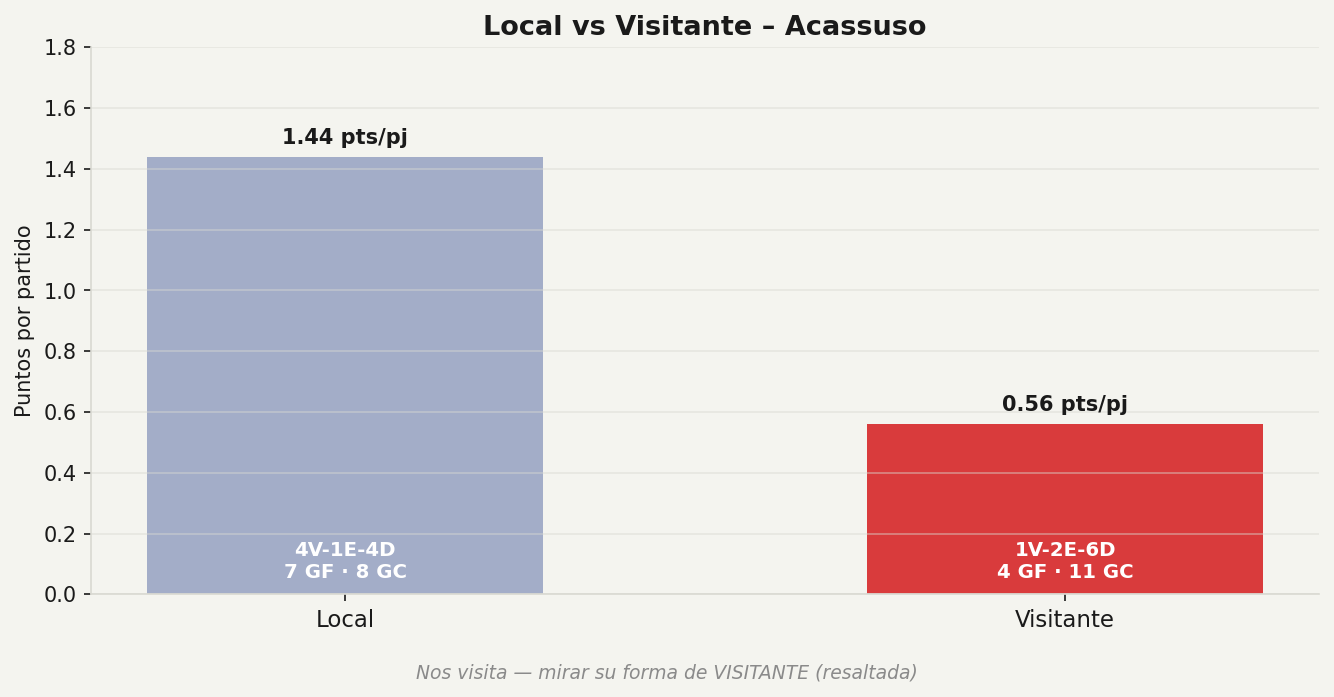
\includegraphics[width=0.80\textwidth]{local_visitante_rival.png}}
  \caption{Rendimiento de Acassuso según la cancha. La columna roja es la que nos toca enfrentar: de visitante rinde menos de la mitad que de local.}
\end{figure}

% --- 2. COMO LLEGA ---
\section*{2. Cómo Llega Acassuso}

Arrancó la temporada con tres victorias seguidas y desde ahí se desplomó: en las siguientes quince fechas ganó apenas dos partidos. La racha reciente es de derrotas y empates, con muchos partidos sin convertir.

En el mano a mano estadístico contra nosotros, los dos equipos se parecen: posesión pareja, pocos remates y poco xG. Ninguno de los dos domina con claridad, así que el partido se va a definir por detalles, pelota parada y errores.

\begin{figure}[htbp]
  \centering
  \fbox{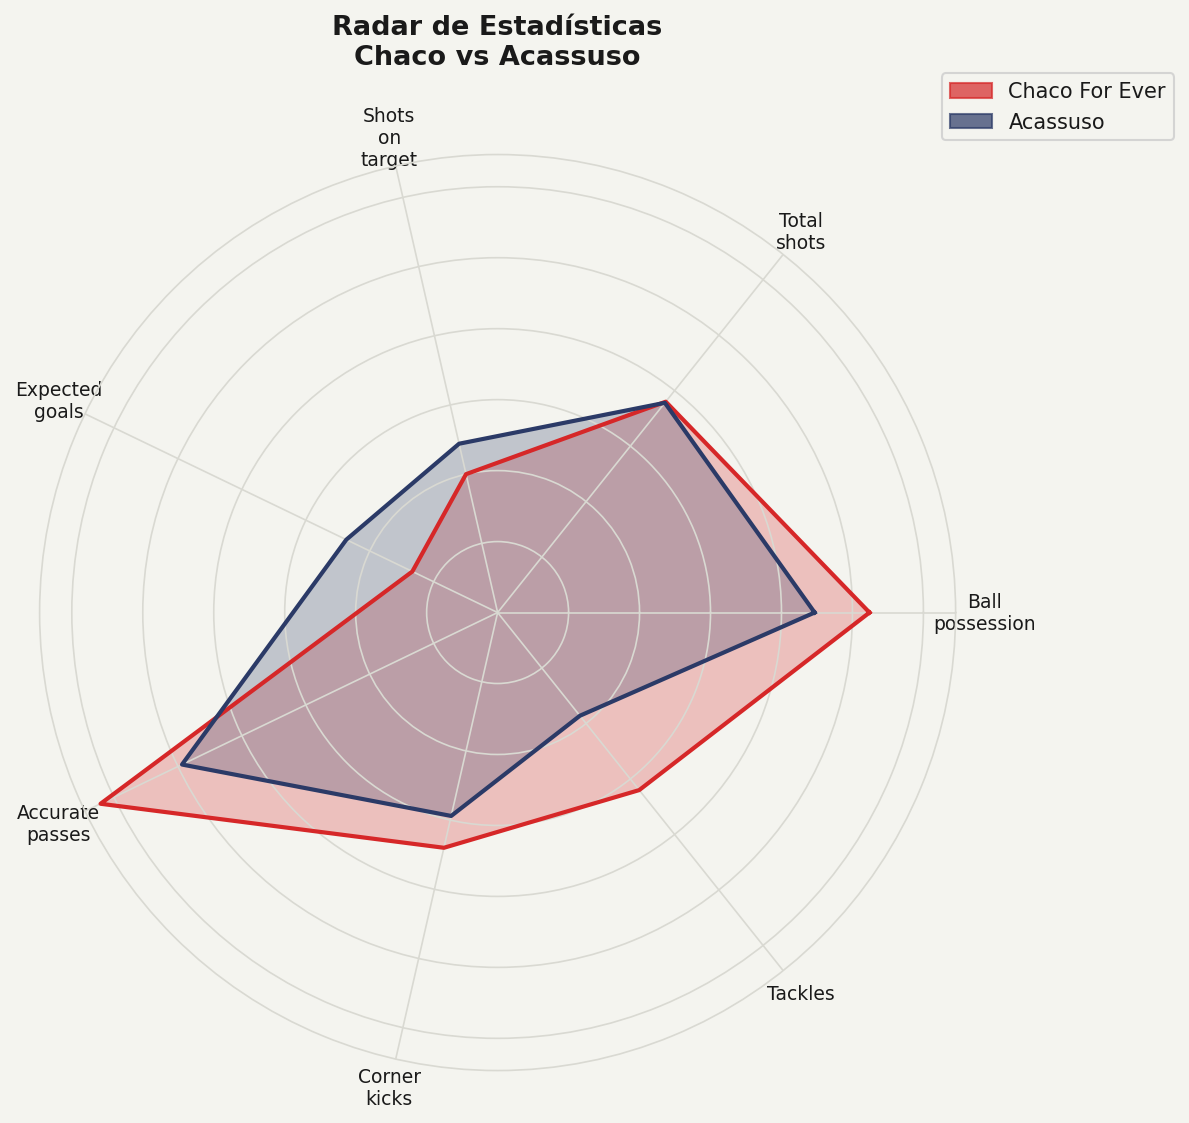
\includegraphics[width=0.66\textwidth]{radar_stats.png}}
  \caption{Perfil estadístico promedio de los dos equipos. Chaco tiene un poco más de posesión y pases; Acassuso patea algo más al arco. Perfiles espejo, sin una ventaja marcada de ninguno.}
\end{figure}

% --- 3. SU EQUIPO ---
\section*{3. Su Equipo}

El once más repetido de Acassuso es un \mA{4-4-2} (lo usó en 10 de 18 fechas), con variantes en 4-2-3-1 y 4-1-4-1. El arquero Monllor es su jugador de mejor promedio (7.32) y jugó los 18 partidos. Adelante, el peligro pasa por dos nombres: \mA{R. Reynoso} (4 goles desde el mediocampo) y \mA{L. Romero} (2 goles y 2 asistencias en solo 9 partidos, y el que nos hizo los dos goles en el primer cruce).

\begin{figure}[htbp]
  \centering
  \fbox{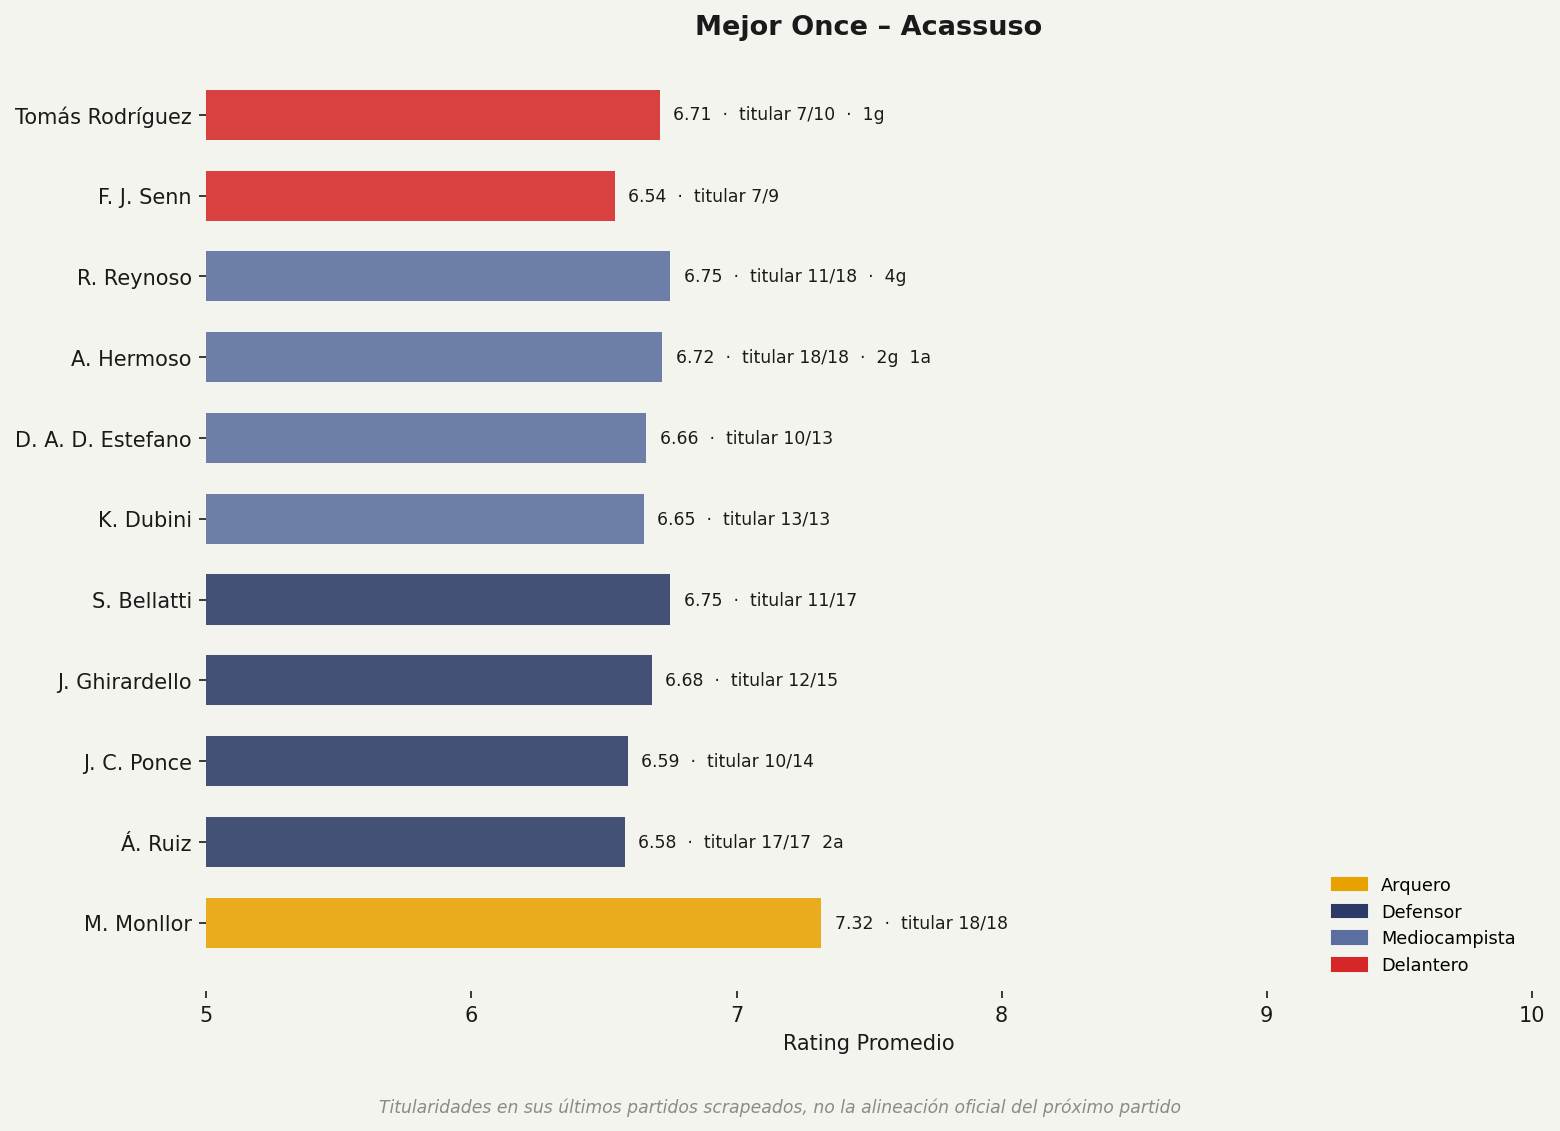
\includegraphics[width=0.72\textwidth]{mejor_once_rival.png}}
  \caption{Once más repetido de Acassuso según titularidades. No es la alineación confirmada, sino con qué equipo suele salir.}
\end{figure}

\begin{figure}[htbp]
  \centering
  \fbox{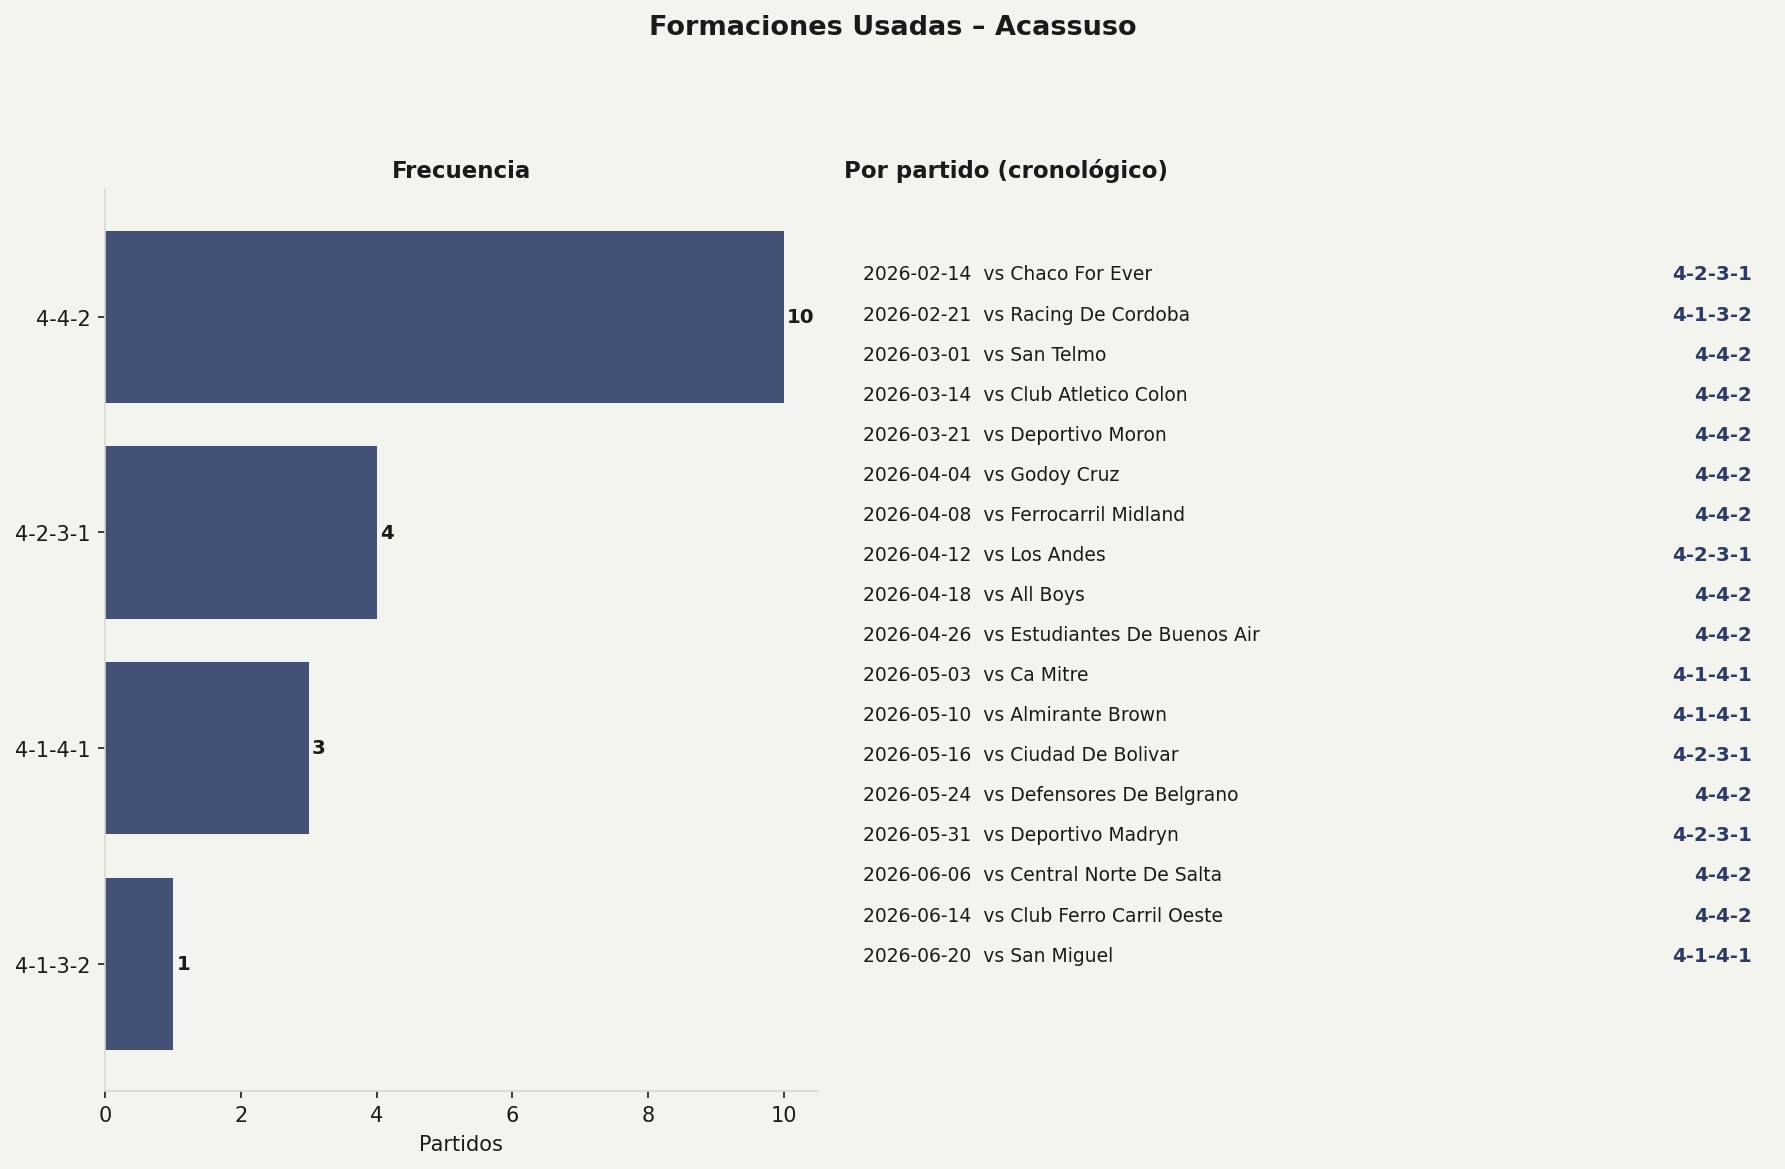
\includegraphics[width=0.90\textwidth]{formaciones_rival.png}}
  \caption{Formaciones usadas fecha a fecha. El 4-4-2 es su base, con ajustes puntuales.}
\end{figure}

\subsection*{Cambió de técnico a mitad de año}

Acassuso no es el mismo proyecto de principio de temporada. \mA{Ángel Darío Lema} dirigió las primeras once fechas y \mA{Tobías Kohan} tomó el equipo en mayo. Kohan es el DT actual. El cambio coincide con el tramo flojo, así que conviene mirar sus últimos partidos más que los del arranque.

\begin{figure}[htbp]
  \centering
  \fbox{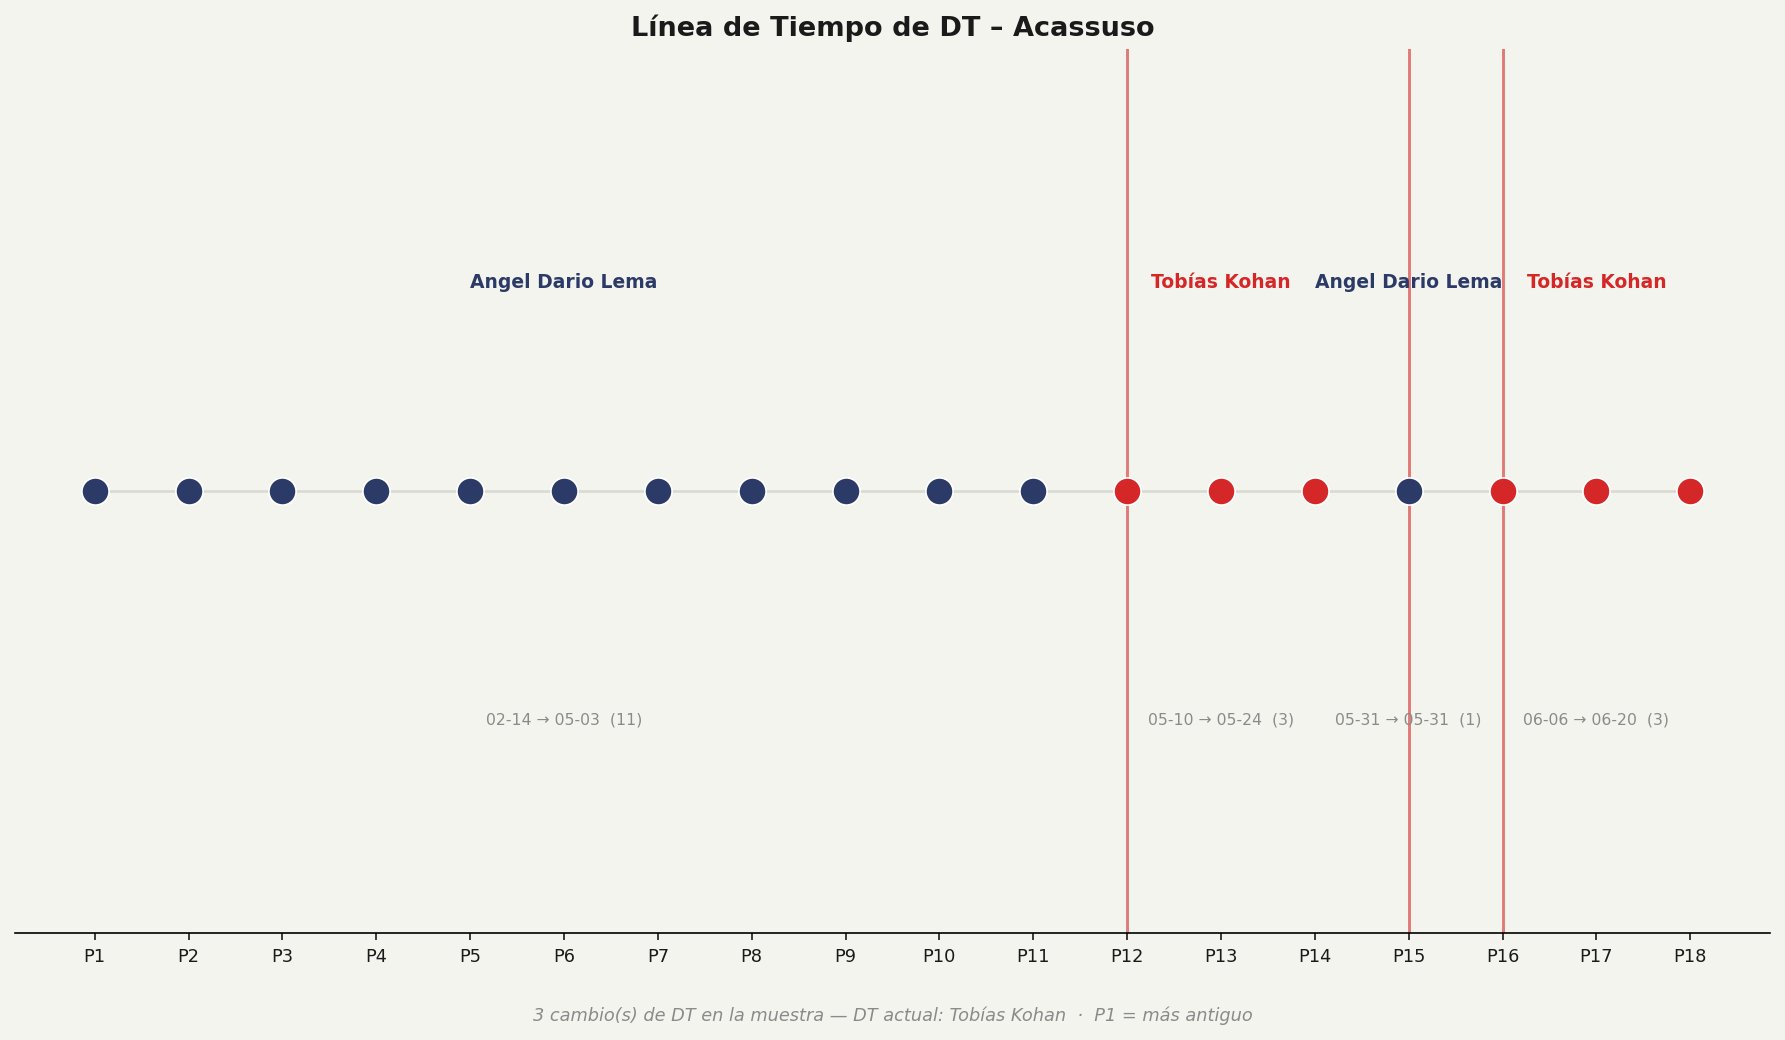
\includegraphics[width=0.92\textwidth]{dt_timeline_rival.png}}
  \caption{Línea de tiempo del cuerpo técnico de Acassuso. El partido suelto de fines de mayo con Lema fue un interinato puntual.}
\end{figure}

% --- 4. ATAQUE ---
\section*{4. Cómo Ataca y Dónde Sufre}

El ataque de Acassuso sale casi todo del centro del área y de dos jugadores. La entropía de sus remates es \mA{36\% del máximo}, un ataque tan leíble como el nuestro. Genera 6.1 de xG en juego abierto en toda la temporada, un número bajo. Si le cerramos el centro y marcamos de cerca a Reynoso y Romero, le cuesta encontrar otra vía.

En defensa muestra una grieta clara: concede \mR{5.22 de xG de córner} y ya recibió 3 goles de esa jugada. Es la invitación a trabajar la pelota parada ofensiva durante la semana.

\begin{figure}[htbp]
  \centering
  \fbox{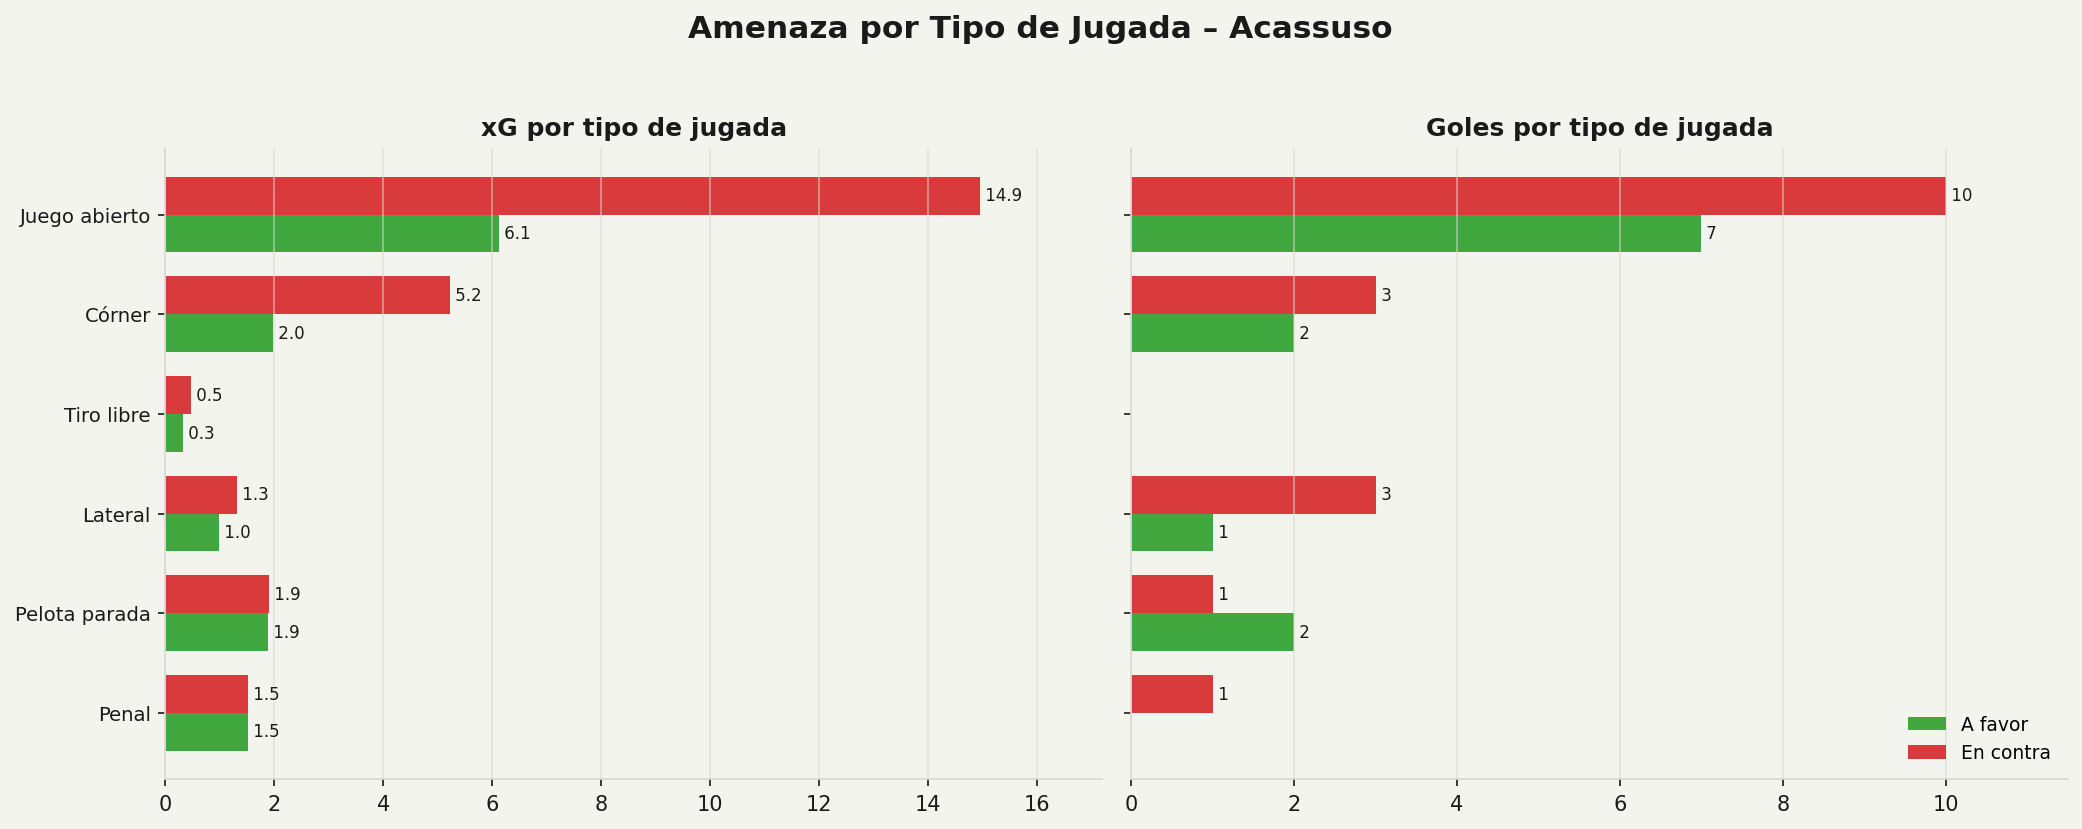
\includegraphics[width=0.92\textwidth]{amenaza_rival.png}}
  \caption{xG y goles de Acassuso por tipo de jugada, a favor y en contra. Genera poco en ataque y sufre en juego abierto y en córner.}
\end{figure}

\begin{figure}[htbp]
  \centering
  \fbox{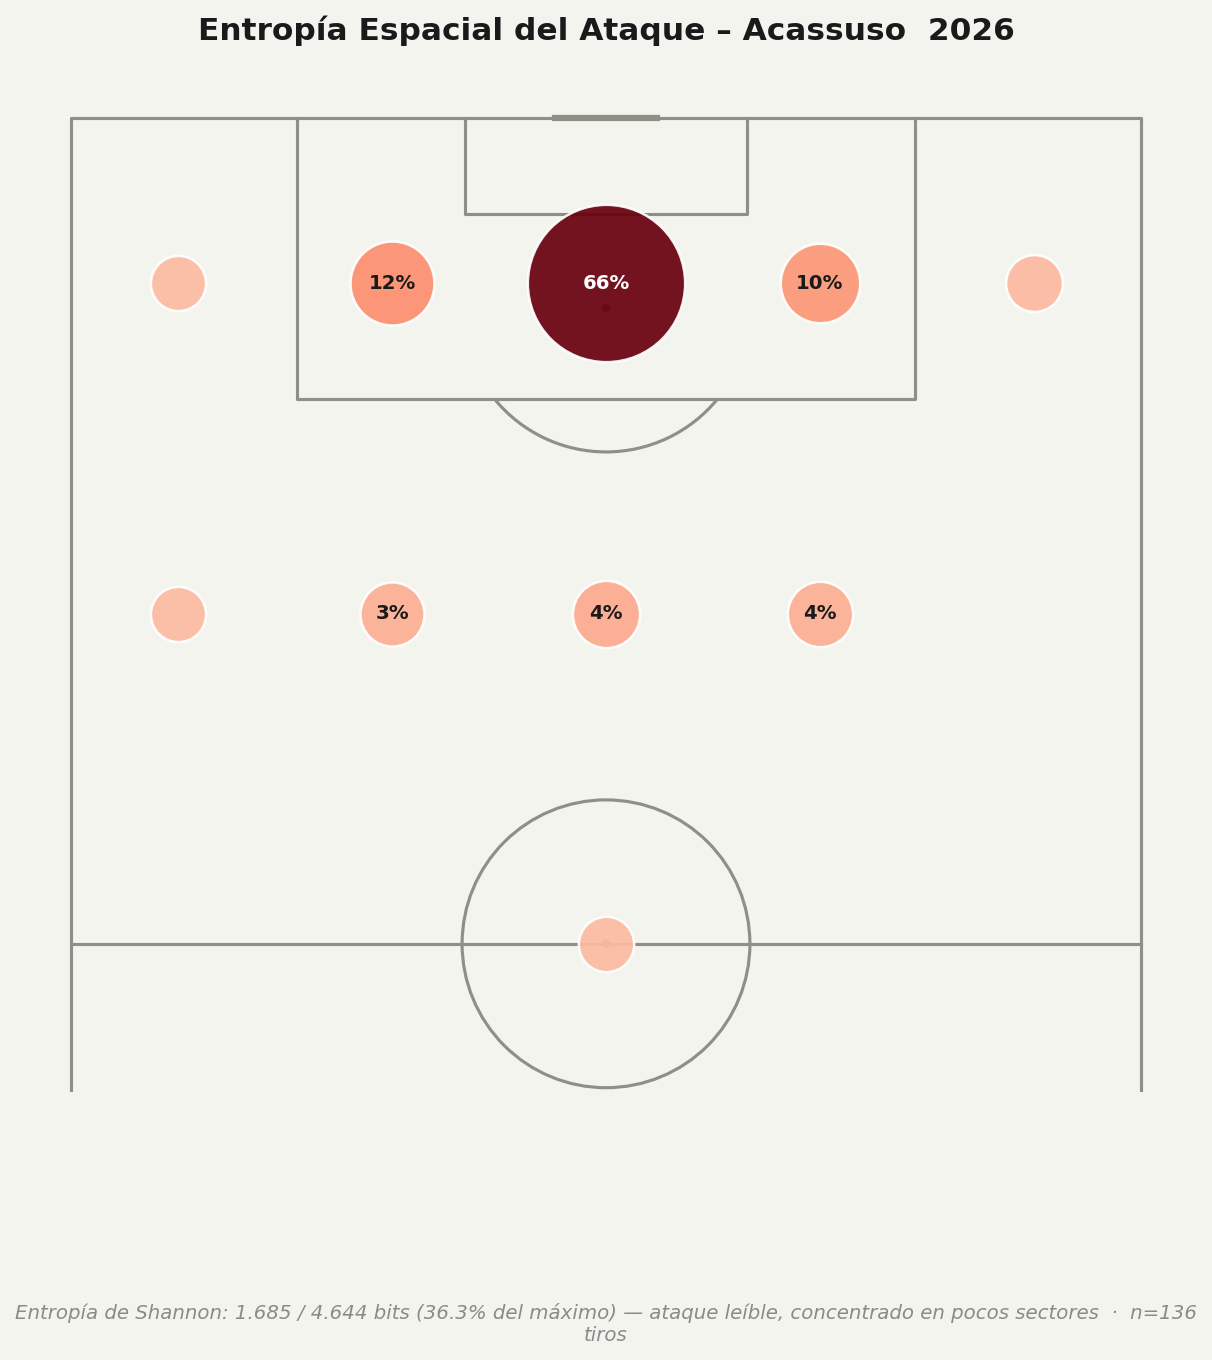
\includegraphics[width=0.55\textwidth]{entropia_rival.png}}
  \caption{Origen de los disparos de Acassuso. La concentración en el centro del área confirma un ataque predecible.}
\end{figure}

% --- 5. DISCIPLINA ---
\section*{5. Disciplina}

Acassuso comete muchas faltas (12.9 por partido) y ve 2.8 amarillas por juego. De cara al partido hay un dato para tener presente: \mR{N. Acosta está a una amarilla de la suspensión} (lleva 4). Es un defensor que suele ser titular, así que una amonestación temprana lo condiciona.

\begin{figure}[htbp]
  \centering
  \fbox{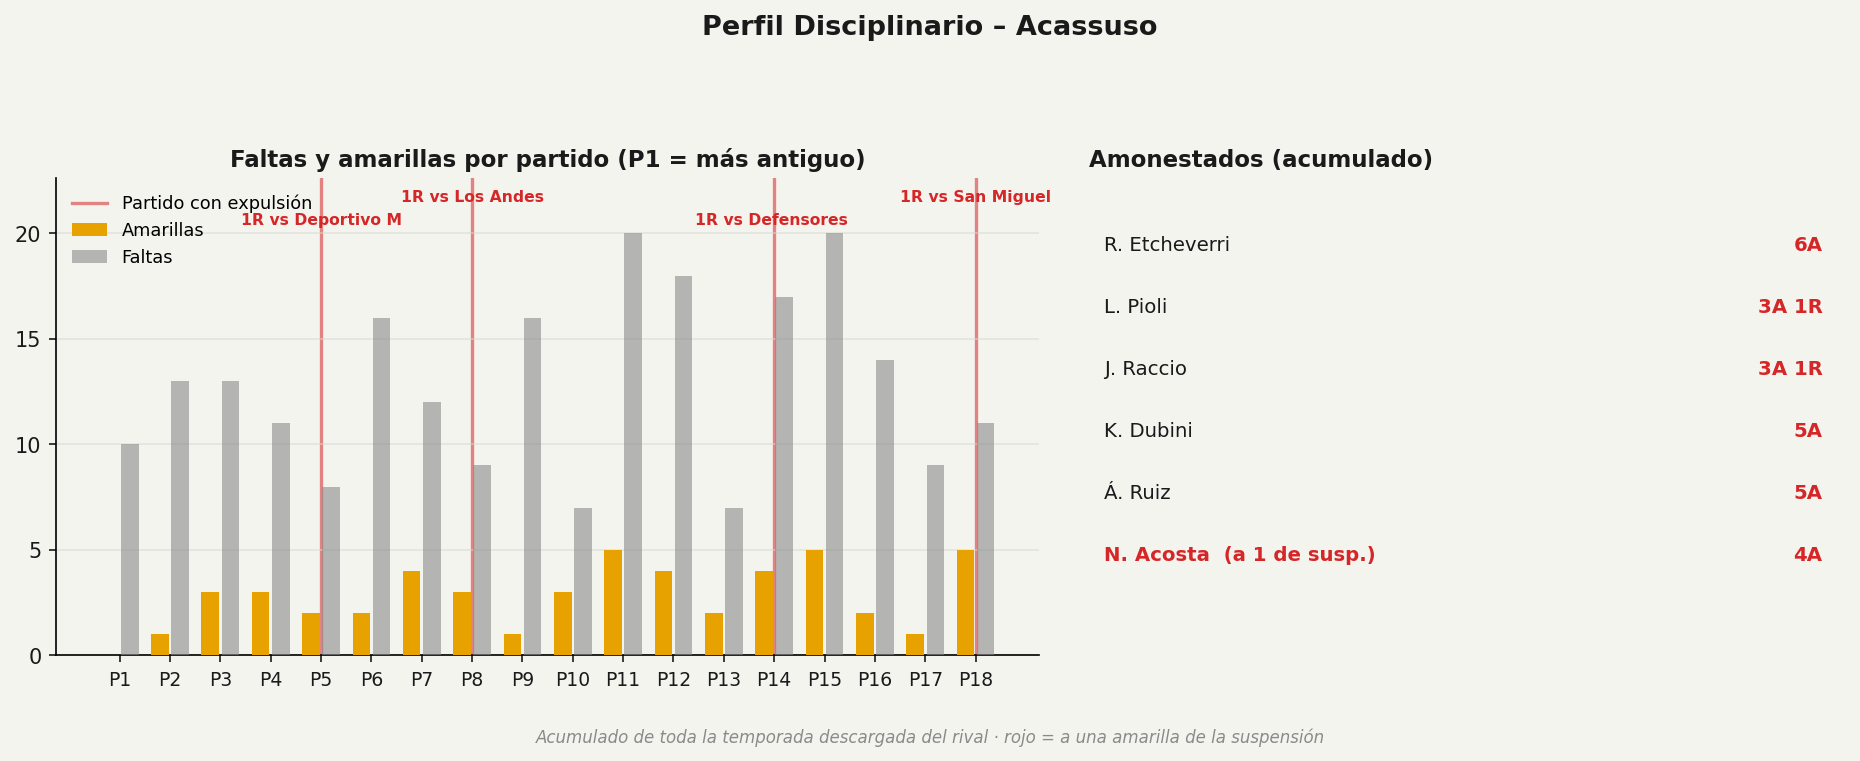
\includegraphics[width=0.98\textwidth]{disciplina_rival.png}}
  \caption{Faltas y amarillas por partido, y acumulado de la temporada. En rojo, el jugador a una amarilla de la suspensión.}
\end{figure}

% --- 6. HISTORIAL Y ULTIMO CRUCE ---
\section*{6. Historial y Último Cruce}

Los equipos se cruzaron una sola vez esta temporada, en la primera fecha, y Acassuso ganó \mR{2-0} de local. Los dos goles fueron de Romero. El partido dejó una señal a corregir: Chaco tuvo más la pelota (53\%) pero generó casi nada (\mR{0.28 de xG contra 1.78} del rival), pateó una sola vez al arco y terminó con un jugador expulsado.

\begin{figure}[htbp]
  \centering
  \fbox{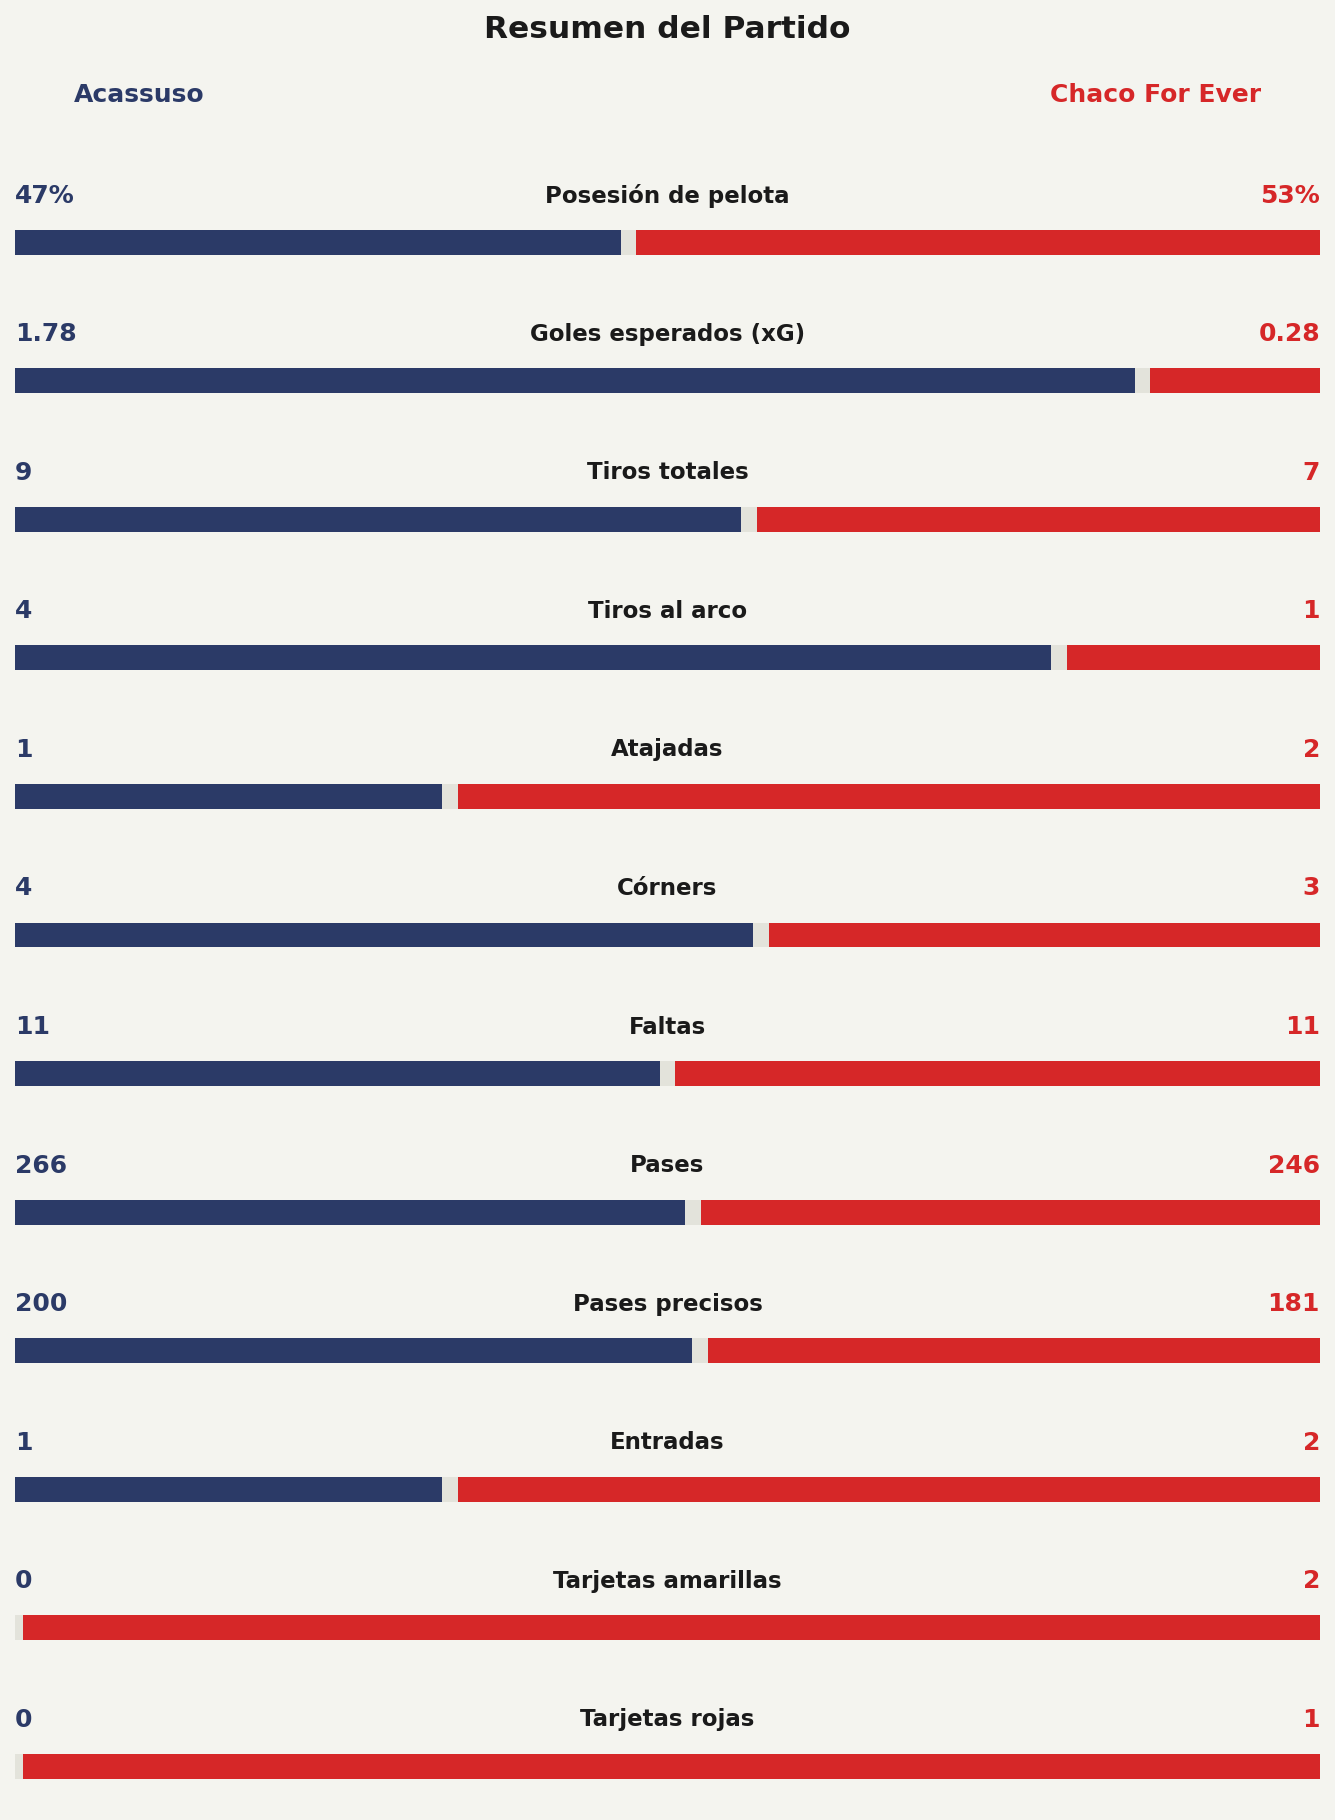
\includegraphics[width=0.52\textwidth]{ultimo_cruce_stats.png}}
  \caption{Estadísticas del 2-0 de la primera fecha. Chaco dominó la posesión sin traducirla en peligro.}
\end{figure}

\begin{figure}[htbp]
  \centering
  \fbox{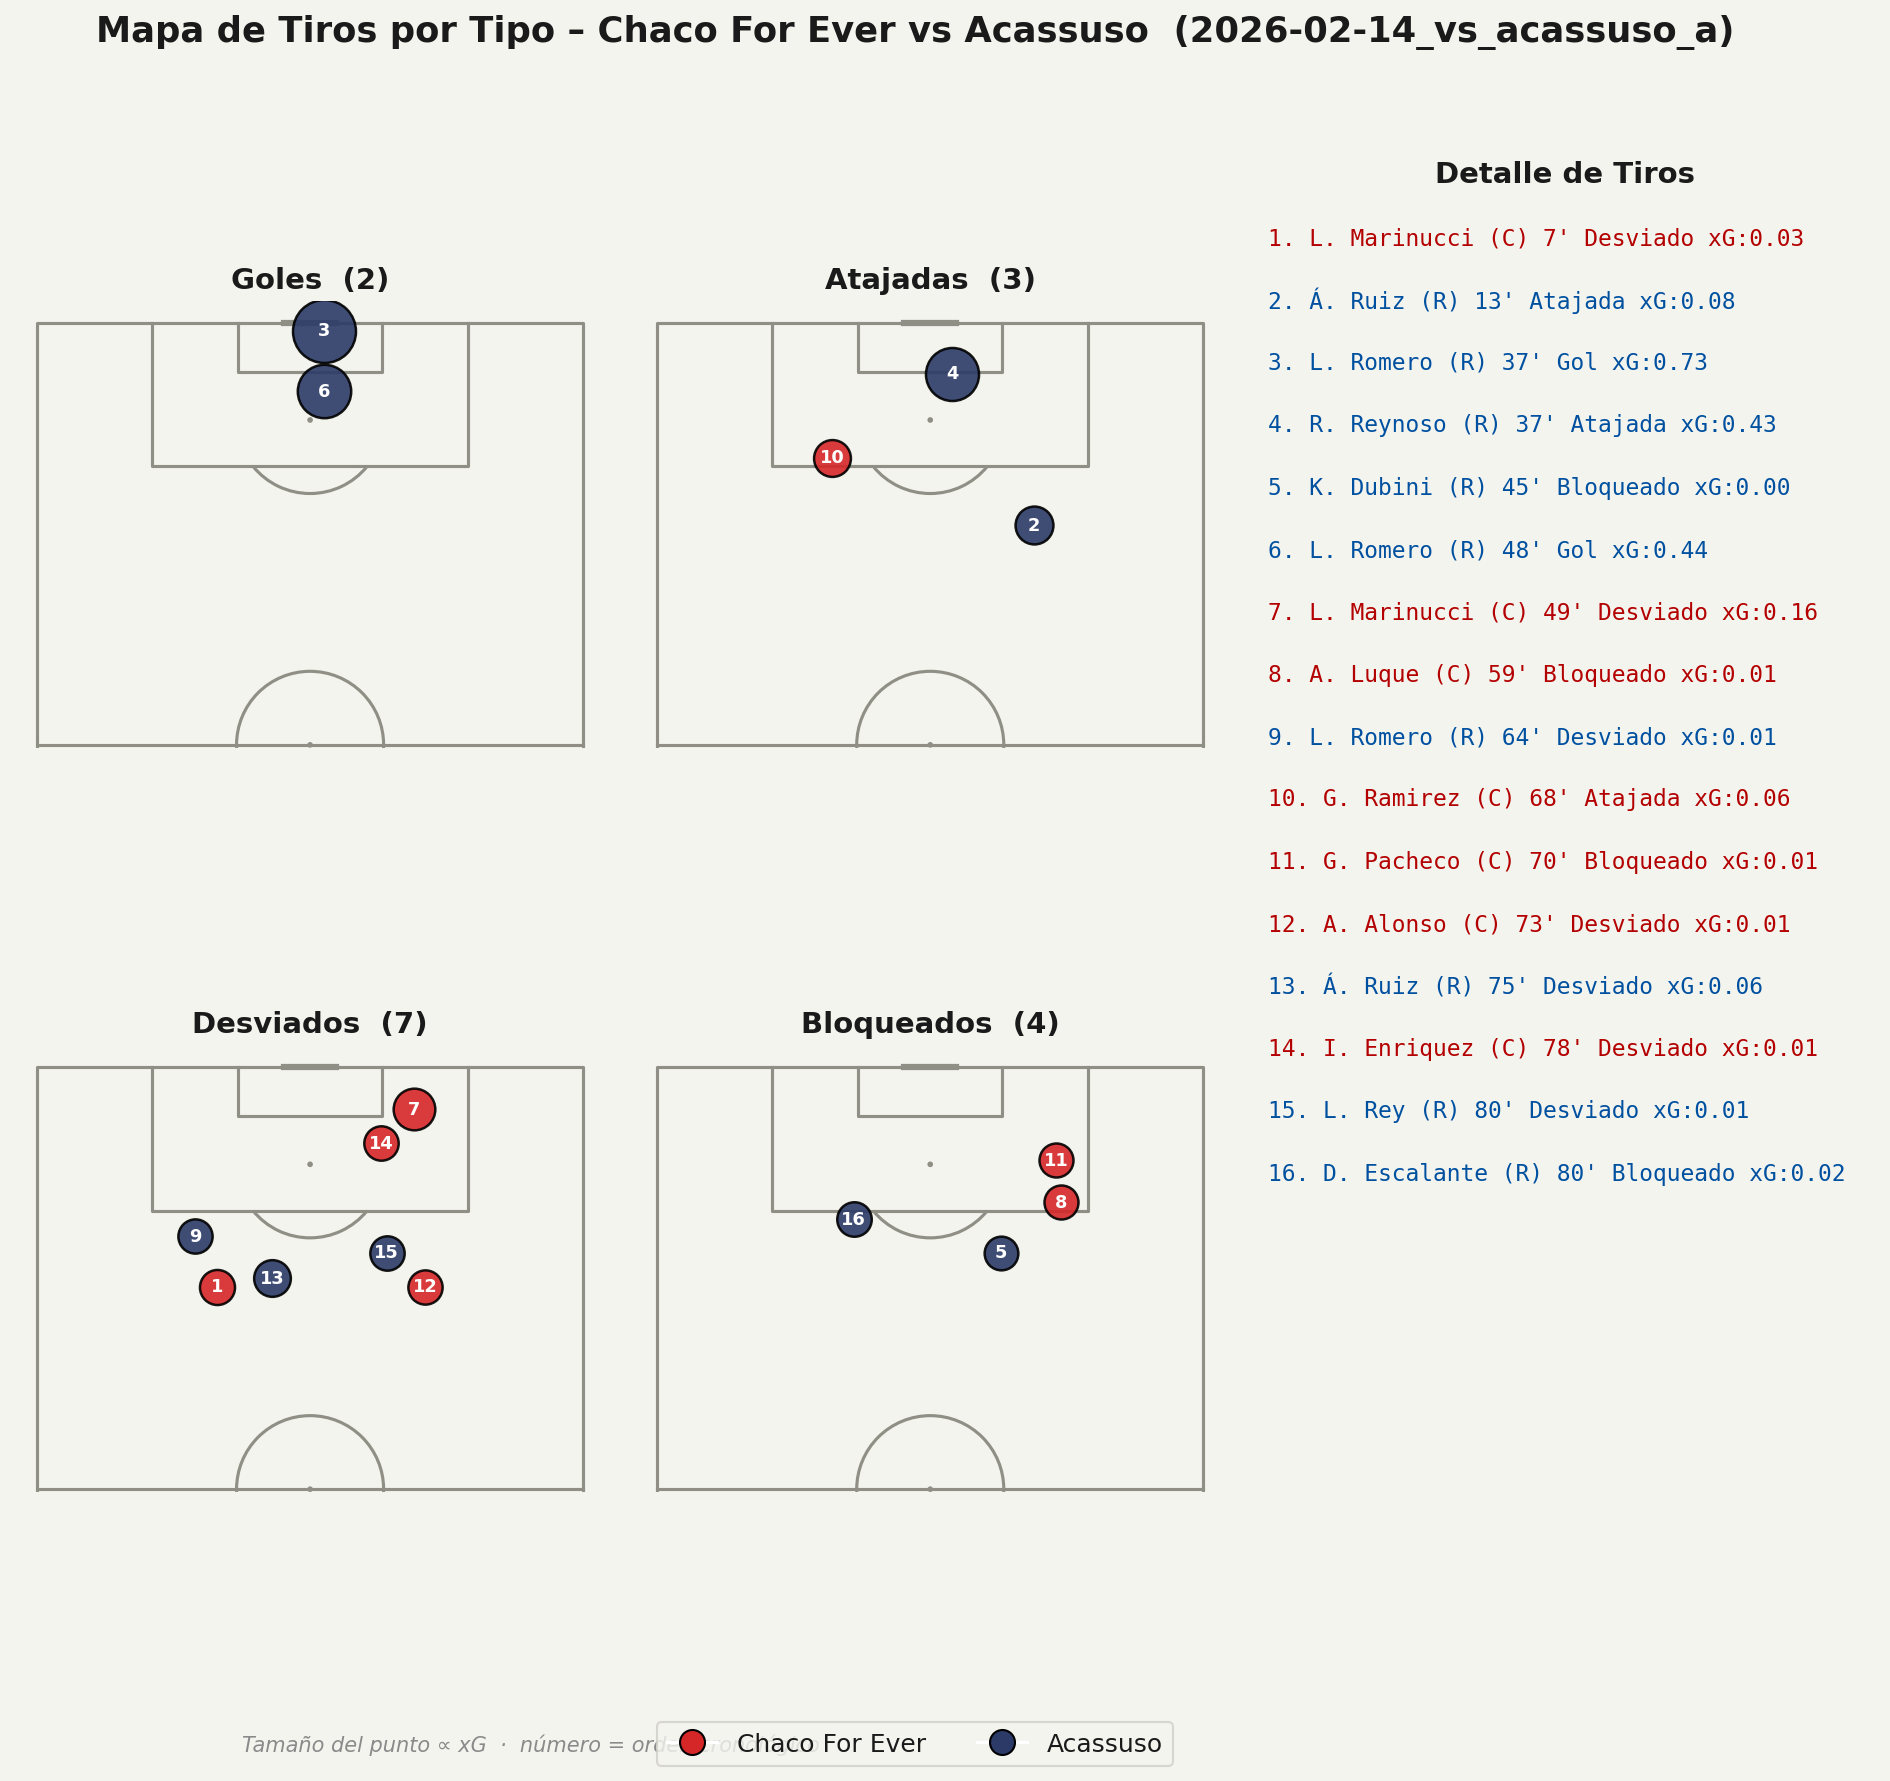
\includegraphics[width=0.98\textwidth]{ultimo_cruce_shotmap.png}}
  \caption{Mapa de tiros de aquel partido: Acassuso generó situaciones claras, Chaco apenas llegó.}
\end{figure}

\begin{figure}[htbp]
  \centering
  \fbox{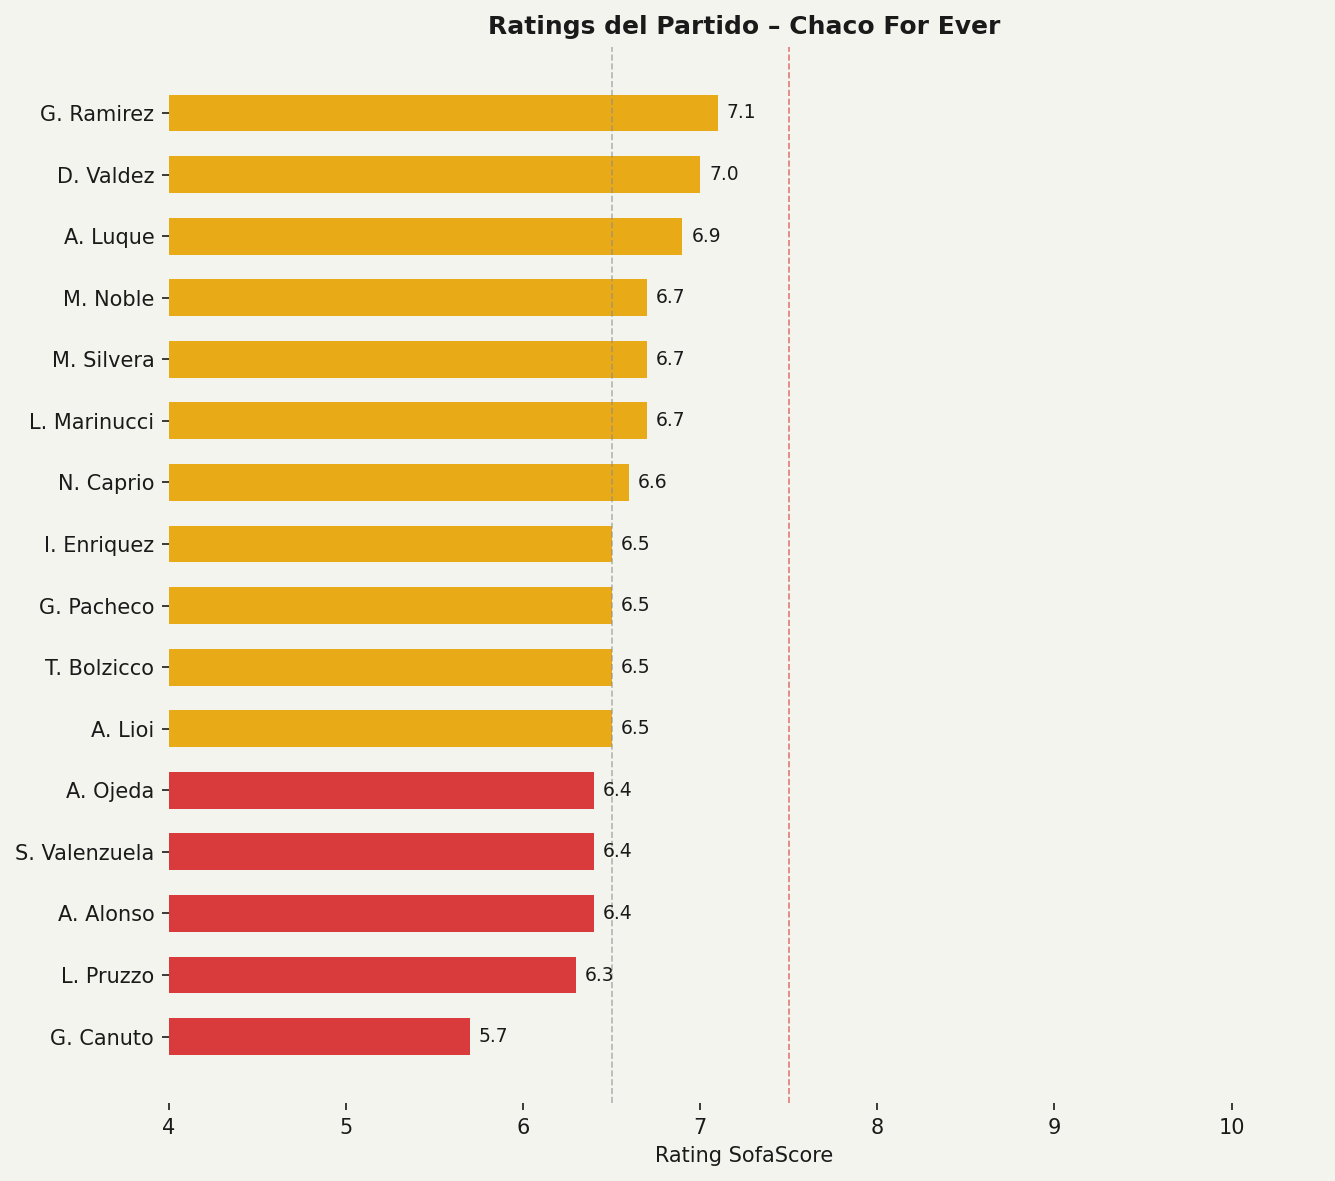
\includegraphics[width=0.98\textwidth]{ultimo_cruce_ratings.png}}
  \caption{Puntajes individuales del primer cruce.}
\end{figure}

\successbox{En una línea}{
  Nos visita un Acassuso flojo de visitante, con ataque pobre y previsible y una grieta en la pelota parada. La revancha del 2-0 pasa por ser efectivos donde en el primer cruce fallamos: convertir la posesión en remates claros y aprovechar el córner.
}

\vspace{2mm}
\hrule
\vspace{1mm}
{\footnotesize\color{darkgray} Datos: pipeline de análisis de Chaco For Ever, temporada 2026. El perfil de Acassuso sale de sus 18 partidos de liga descargados. El DT se obtuvo del endpoint de entrenadores de la fuente.}

\end{document}
